\documentclass[12pt,a4paper]{article}
\usepackage[utf8]{inputenc}
\usepackage[english]{babel}
\usepackage{geometry}
\usepackage{fancyhdr}
\usepackage{graphicx}
\usepackage{longtable}
\usepackage{array}
\usepackage{booktabs}
\usepackage{xcolor}
\usepackage{hyperref}
\usepackage{listings}
\usepackage{enumitem}
\usepackage{caption}
\usepackage{float} % for [H] placement
\geometry{margin=1in}
\pagestyle{fancy}
\fancyhf{}
\rhead{\thepage}
\lhead{HIV Clinic RDS}

\title{\textbf{Requirement \& Design Specification\\HIV Clinic Appointment Booking System}}
\author{Version: 2.0}
\date{January 2025}

\begin{document}

\maketitle
\thispagestyle{empty}

\newpage

\section*{Record of Changes}

\begin{table}[h!]
\centering
\renewcommand{\arraystretch}{1.5}
\begin{tabular}{|c|c|c|c|p{7.5cm}|}
\hline
\textbf{Version} & \textbf{Date} & \textbf{A* M, D} & \textbf{In charge} & \textbf{Change Description} \\
\hline
V1.0 & 28/6 & A & KhoaDDSE196260 & 
Create document \newline
Add requirements, Add actors (1.1) \newline
Design Specification\\
\hline
V1.0 & 28/6 & A & TuanTMSE192397 & 
Add descriptions for guest and admin (1.2.b) \newline
Authentication \& User Management (2.1) \\
\hline
V1.0 & 28/6 & A & DatNTSE194083 & 
Add Use Case Diagram (1.2.a)\newline 
Add Requirement Speciality
\\
\hline
V1.0 & 28/6 & A & AnPPSE196260 & 
Add Use case Table(1.2.1)
Add ScreenFlow Diagram (2.1) \newline
(2.2) Screen Descriptions, Appendix\newline 
Add Requirement Speciality\\
\hline
V2.0 & Jan 2025 & M & Background Agent & 
Updated to use definitive 27 use cases from evaluation \newline
Aligned with HIV_Clinic_Use_Cases.md \newline
Corrected use case specifications and design details\\
\hline
\end{tabular}
\caption{Version Change Log}
\label{tab:version-log}
\end{table}

\textit{*A - Added M - Modified D - Deleted}

\newpage

\tableofcontents

\newpage

\section{Overview}

\subsection{User Requirements}

\subsubsection{Actors}

The HIV Clinic Appointment Booking System involves five main actors who interact with the system to perform various healthcare-related tasks. The system follows an inheritance model where all authenticated users inherit the basic capabilities of unauthenticated users.

\subsection{Actor Description}

\begin{longtable}{|c||c|p{9cm}|}
\hline
\textbf{No} & \textbf{Actor} & \textbf{Description} \\
\hline
01 & Unauthenticated User & The base actor with public access capabilities. Can browse public website content, register for accounts, and login to the system. All other actors inherit these capabilities. \\
\hline
02 & Patient & A registered and authenticated user who receives HIV care. Inherits all base capabilities plus: can manage appointments, view personal medical records and ARV treatments, receive notifications, and access personalized dashboard. \\
\hline
03 & Doctor & A registered and authenticated medical professional. Inherits all base capabilities plus: can manage professional availability, handle patient appointments and consultations, prescribe and monitor ARV treatments, and manage patient notifications. \\
\hline
04 & Admin & A privileged user responsible for system administration. Inherits all base capabilities plus: manages user accounts across the system, handles user account operations, and monitors appointment oversight. \\
\hline
05 & Manager & An authenticated user with operational oversight capabilities. Inherits all base capabilities plus: views comprehensive analytics, manages patient and doctor records, oversees ARV treatment programs, and handles data export operations. \\
\hline
\end{longtable}

\subsubsection{Use Cases}

\paragraph{a. Diagram(s)}

\begin{figure}[H]
\centering
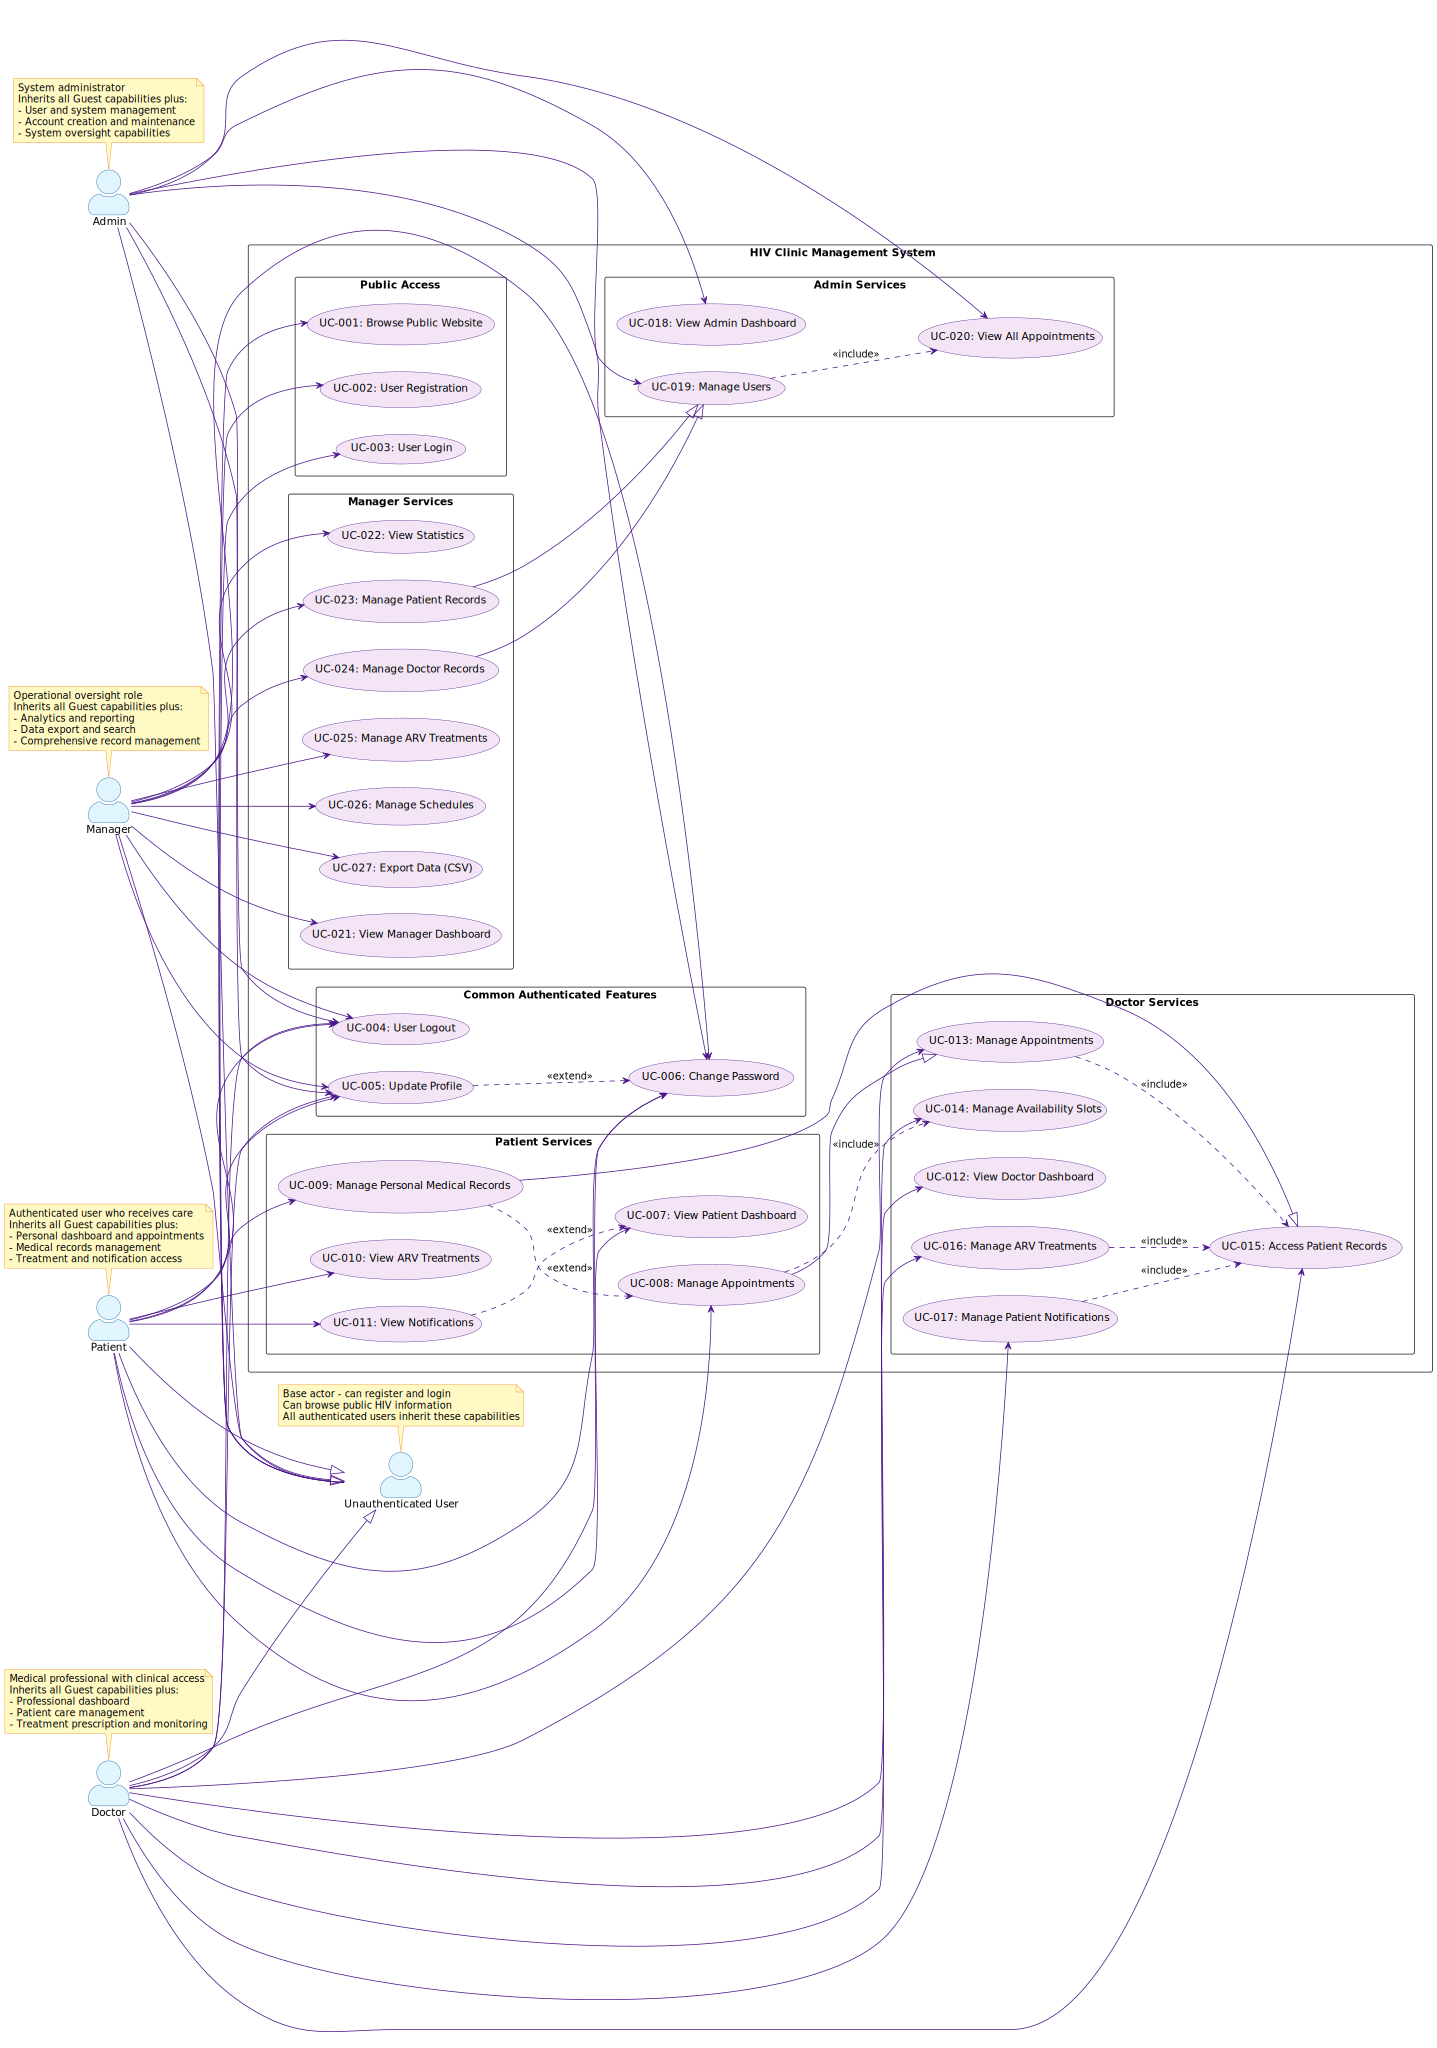
\includegraphics[width=0.9\textwidth]{diagrams/use_case_diagram.svg}
\caption{HIV Clinic Management System Use Case Diagram}
\label{fig:use-case-diagram}
\end{figure}

The system provides 27 comprehensive use cases organized by actor roles, following an inheritance model where authenticated users inherit public access capabilities while adding role-specific functionalities for HIV clinic management.

\paragraph{b. Use Case Descriptions}

\begin{longtable}{|p{1cm}|p{3cm}|p{3cm}|p{7cm}|}
\hline
\textbf{ID} & \textbf{Feature} & \textbf{Use Case} & \textbf{Use Case Description} \\
\hline
\multicolumn{4}{|c|}{\textbf{Unauthenticated User (Base Capabilities)}} \\
\hline
UC-001 & Public Information & Browse Public Website & View HIV information, educational content, and blog posts accessible to all visitors \\
\hline
UC-002 & Account Management & User Registration & Patients and doctors can register for new accounts with role-based system access \\
\hline
UC-003 & Authentication & User Login & Authenticate using username/password with JWT token-based security \\
\hline
\multicolumn{4}{|c|}{\textbf{Authenticated User (Common Capabilities)}} \\
\hline
UC-004 & Authentication & User Logout & Secure session termination and cleanup for all authenticated users \\
\hline
UC-005 & Profile Management & Update Profile & Manage personal information, contact details, profile images, and privacy settings \\
\hline
UC-006 & Security & Change Password & Password modification with validation and security checks \\
\hline
\multicolumn{4}{|c|}{\textbf{Patient Services}} \\
\hline
UC-007 & Dashboard & View Patient Dashboard & Overview of appointments, treatments, and personal health statistics \\
\hline
UC-008 & Appointment & Manage Appointments & Book, view, and cancel appointments with available doctors \\
\hline
UC-009 & Medical Records & Manage Personal Medical Records & View and update personal medical records and information \\
\hline
UC-010 & HIV Treatment & View ARV Treatments & View HIV antiretroviral treatment regimens and status \\
\hline
UC-011 & Communication & View Notifications & Receive and view system notifications and reminders \\
\hline
\multicolumn{4}{|c|}{\textbf{Doctor Services}} \\
\hline
UC-012 & Dashboard & View Doctor Dashboard & Professional dashboard with patient appointments and notifications \\
\hline
UC-013 & Appointment & Manage Appointments & View, manage patient appointments, and update appointment status \\
\hline
UC-014 & Scheduling & Manage Availability Slots & Create, update, and delete availability time slots for appointments \\
\hline
UC-015 & Patient Care & Access Patient Records & View comprehensive patient medical records during consultations \\
\hline
UC-016 & HIV Treatment & Manage ARV Treatments & Prescribe and monitor HIV antiretroviral treatments \\
\hline
UC-017 & Communication & Manage Patient Notifications & Send notifications, view history, and manage templates \\
\hline
\multicolumn{4}{|c|}{\textbf{Admin Services}} \\
\hline
UC-018 & Dashboard & View Admin Dashboard & System-wide administrative dashboard with user management tools \\
\hline
UC-019 & User Management & Manage Users & Comprehensive user management including account creation, status toggling, and password resets \\
\hline
UC-020 & System Oversight & View All Appointments & System-wide appointment oversight and monitoring \\
\hline
\multicolumn{4}{|c|}{\textbf{Manager Services}} \\
\hline
UC-021 & Dashboard & View Manager Dashboard & Operational dashboard with comprehensive analytics, data export, and clinic statistics \\
\hline
UC-022 & Analytics & View Statistics & Comprehensive clinic statistics and performance metrics \\
\hline
UC-023 & Operations & Manage Patient Records & Oversight of patient records, including search and detailed views \\
\hline
UC-024 & Operations & Manage Doctor Records & Oversight of doctor records, including search and detailed views \\
\hline
UC-025 & Treatment Oversight & Manage ARV Treatments & Monitor ARV treatment programs across the clinic \\
\hline
UC-026 & Scheduling & Manage Schedules & Oversee clinic scheduling and appointment distribution \\
\hline
UC-027 & Data Management & Export Data (CSV) & Export clinic data in CSV format for reporting and analysis \\
\hline
\end{longtable}

\subsection{Overall Functionalities}

\subsubsection{Screen Flow}

The HIV Clinic system provides role-based screen flows ensuring appropriate access to sensitive medical information:

\begin{figure}[H]
    \centering
    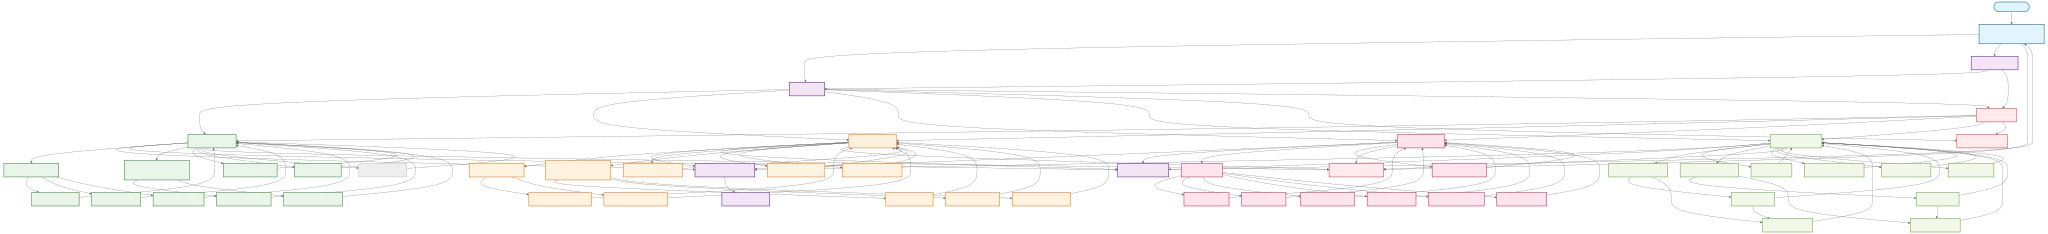
\includegraphics[width=0.9\textwidth]{diagrams/user_interface_flow.svg}
    \caption{Overall Screen Flow}
    \label{fig:screen-flow}
\end{figure}

\subsubsection{Screen Descriptions}

\renewcommand{\arraystretch}{1.4}
\begin{longtable}{|c|c|c|p{8.5cm}|}
\hline
\textbf{\#} & \textbf{Feature} & \textbf{Screen} & \textbf{Description} \\
\hline
\endfirsthead

\hline
\textbf{\#} & \textbf{Feature} & \textbf{Screen} & \textbf{Description} \\
\hline
\endhead

1 & Authentication & HOME PAGE & The landing page of the system. Includes brief introduction, access to login/register, blog, and HIV educational content. \\
\hline
2 & Authentication & Register Page & Allows users (patients, doctors) to create new accounts with basic info and email verification. \\
\hline
3 & Authentication & LOGIN PAGE & Login page for all users. After successful login, users are routed to their respective dashboard based on role. \\
\hline
4 & Information & Information Page & Displays HIV clinic information and services. Accessible from Home Page without login. \\
\hline
5 & Blog & Blog Page & HIV health education blogs and articles available for reading from the Home Page. \\
\hline
6 & Dashboard & Patient Dashboard & Main landing screen after login for patients. Central hub for accessing medical features and appointments. \\
\hline
7 & Dashboard & Doctor Dashboard & Professional dashboard for doctors showing patient appointments, availability, and notifications. \\
\hline
8 & Dashboard & Admin Dashboard & Administrative dashboard for managing users, viewing system statistics, and monitoring appointments. \\
\hline
9 & Dashboard & Manager Dashboard & Operational dashboard with comprehensive analytics, data export, and clinic statistics. \\
\hline
10 & Appointment & Appointment Booking & Patient interface for booking appointments with available doctors and time slots. \\
\hline
11 & Medical Records & Patient Records & Interface for viewing and managing personal medical records, including HIV treatment history. \\
\hline
12 & Treatment & ARV Management & Specialized interface for managing HIV antiretroviral treatments and monitoring adherence. \\
\hline
\end{longtable}

\section{Use Case Specifications}

\subsection{UC-001 – Browse Public Website}

\renewcommand{\arraystretch}{1.5}
\begin{longtable}{|p{4.5cm}|p{10.5cm}|}
\hline
\textbf{UC ID and Name:} & UC-001 – Browse Public Website \\
\hline
\textbf{Created By:} & System Analyst \\
\hline
\textbf{Date Created:} & January 2025 \\
\hline
\textbf{Primary Actor:} & Unauthenticated User \\
\hline
\textbf{Secondary Actors:} & None \\
\hline
\textbf{Description:} & Users can view HIV information, educational content, and blog posts without requiring authentication \\
\hline
\textbf{Trigger:} & User accesses the website homepage or navigation menu \\
\hline
\textbf{Preconditions:} &
\begin{itemize}
  \item The system is online and accessible
  \item Public content is available in the system
\end{itemize} \\
\hline
\textbf{Postconditions:} &
\begin{itemize}
  \item Public HIV information and content is displayed
  \item User can navigate through available public pages
\end{itemize} \\
\hline
\textbf{Normal Flow:} &
\begin{enumerate}
  \item User opens the website
  \item System displays homepage with HIV clinic information
  \item User navigates through public content sections
  \item User can read educational content and blog posts
\end{enumerate} \\
\hline
\textbf{Alternative Flows:} & 
\textbf{AF-1:} User accesses specific public pages directly via URL \\
\hline
\textbf{Exceptions:} &
\begin{itemize}
  \item EX-1: If public content is unavailable, system displays maintenance message
\end{itemize} \\
\hline
\textbf{Business Rules:} &
\begin{itemize}
  \item BR-001: Public content must be accessible without authentication
  \item BR-002: HIV educational content must be medically accurate
\end{itemize} \\
\hline
\textbf{Assumptions:} &
\begin{itemize}
  \item Public content is regularly updated and maintained
\end{itemize} \\
\hline
\textbf{Priority:} & High \\
\hline
\textbf{Frequency of Use:} & High \\
\hline
\end{longtable}

\subsection{UC-002 – User Registration}

\renewcommand{\arraystretch}{1.5}
\begin{longtable}{|p{4.5cm}|p{10.5cm}|}
\hline
\textbf{UC ID and Name:} & UC-002 – User Registration \\
\hline
\textbf{Created By:} & System Analyst \\
\hline
\textbf{Date Created:} & January 2025 \\
\hline
\textbf{Primary Actor:} & Unauthenticated User \\
\hline
\textbf{Secondary Actors:} & System \\
\hline
\textbf{Description:} & New users (patients and doctors) can create accounts with role-based access to the HIV clinic system \\
\hline
\textbf{Trigger:} & User clicks "Register" from homepage or login page \\
\hline
\textbf{Preconditions:} &
\begin{itemize}
  \item User is not currently logged in
  \item Registration system is operational
\end{itemize} \\
\hline
\textbf{Postconditions:} &
\begin{itemize}
  \item New user account is created in the system
  \item User receives confirmation notification
  \item User can login with new credentials
\end{itemize} \\
\hline
\textbf{Normal Flow:} &
\begin{enumerate}
  \item User accesses registration form
  \item User provides required information (name, email, phone, role)
  \item User creates username and password
  \item System validates input data
  \item System creates new user account
  \item System sends confirmation notification
\end{enumerate} \\
\hline
\textbf{Alternative Flows:} &
\textbf{AF-1:} Email already exists → System shows error and suggests login \\
\textbf{AF-2:} Invalid data format → System highlights errors for correction \\
\hline
\textbf{Exceptions:} &
\begin{itemize}
  \item EX-1: System error during registration → Show error message and retry option
\end{itemize} \\
\hline
\textbf{Business Rules:} &
\begin{itemize}
  \item BR-003: Email addresses must be unique in the system
  \item BR-004: Passwords must meet security requirements
  \item BR-005: Doctor registrations require additional verification
\end{itemize} \\
\hline
\textbf{Assumptions:} &
\begin{itemize}
  \item Users provide accurate contact information
\end{itemize} \\
\hline
\textbf{Priority:} & High \\
\hline
\textbf{Frequency of Use:} & Medium \\
\hline
\end{longtable}

\subsection{UC-003 – User Login}

\renewcommand{\arraystretch}{1.5}
\begin{longtable}{|p{4.5cm}|p{10.5cm}|}
\hline
\textbf{UC ID and Name:} & UC-003 – User Login \\
\hline
\textbf{Created By:} & System Analyst \\
\hline
\textbf{Date Created:} & January 2025 \\
\hline
\textbf{Primary Actor:} & Unauthenticated User \\
\hline
\textbf{Secondary Actors:} & System \\
\hline
\textbf{Description:} & Existing users authenticate using username/password with JWT token-based security \\
\hline
\textbf{Trigger:} & User accesses login page and submits credentials \\
\hline
\textbf{Preconditions:} &
\begin{itemize}
  \item A registered account exists
  \item The user is not currently logged in
  \item Authentication system is operational
\end{itemize} \\
\hline
\textbf{Postconditions:} &
\begin{itemize}
  \item The user is authenticated
  \item The user is redirected to their personal dashboard
  \item Login activity is logged for security
\end{itemize} \\
\hline
\textbf{Normal Flow:} &
\begin{enumerate}
  \item User enters username/email and password
  \item The system validates the credentials
  \item System generates JWT token
  \item User is redirected to appropriate dashboard based on role
  \item System logs successful login
\end{enumerate} \\
\hline
\textbf{Alternative Flows:} &
\textbf{AF-1:} Invalid credentials → System shows error message \\
\textbf{AF-2:} Account disabled → System shows account status message \\
\hline
\textbf{Exceptions:} &
\begin{itemize}
  \item EX-1: Multiple failed attempts → Account temporarily locked
  \item EX-2: System authentication error → Show retry option
\end{itemize} \\
\hline
\textbf{Business Rules:} &
\begin{itemize}
  \item BR-006: Maximum 3 failed login attempts before temporary account lockout
  \item BR-007: Session timeout after 2 hours of inactivity
  \item BR-008: All login attempts must be logged for security audit
\end{itemize} \\
\hline
\textbf{Assumptions:} &
\begin{itemize}
  \item The account is active and verified
  \item The user provides correct credentials
\end{itemize} \\
\hline
\textbf{Priority:} & High \\
\hline
\textbf{Frequency of Use:} & High \\
\hline
\end{longtable}

\subsection{UC-008 – Manage Appointments}

\renewcommand{\arraystretch}{1.5}
\begin{longtable}{|p{4.5cm}|p{10.5cm}|}
\hline
\textbf{UC ID and Name:} & UC-008 – Manage Appointments \\
\hline
\textbf{Created By:} & System Analyst \\
\hline
\textbf{Date Created:} & January 2025 \\
\hline
\textbf{Primary Actor:} & Patient \\
\hline
\textbf{Secondary Actors:} & System, Doctor \\
\hline
\textbf{Description:} & Patients can book, view, and cancel appointments with available doctors \\
\hline
\textbf{Trigger:} & Patient accesses appointment management section \\
\hline
\textbf{Preconditions:} &
\begin{itemize}
  \item Patient is logged in to the system
  \item At least one doctor has available appointment slots
\end{itemize} \\
\hline
\textbf{Postconditions:} &
\begin{itemize}
  \item Appointment is successfully booked, viewed, or cancelled
  \item Doctor and patient receive appropriate notifications
  \item Appointment status is updated in the system
\end{itemize} \\
\hline
\textbf{Normal Flow:} &
\textbf{Booking:}
\begin{enumerate}
  \item Patient selects doctor from available list
  \item Patient chooses available date and time slot
  \item Patient provides appointment notes (optional)
  \item System creates appointment and updates availability
  \item System sends confirmation to patient and doctor
\end{enumerate}
\textbf{Viewing:}
\begin{enumerate}
  \item Patient accesses appointment list
  \item System displays past, current, and future appointments
  \item Patient can view appointment details
\end{enumerate}
\textbf{Cancelling:}
\begin{enumerate}
  \item Patient selects appointment to cancel
  \item Patient provides cancellation reason
  \item System cancels appointment and frees time slot
  \item System notifies doctor of cancellation
\end{enumerate} \\
\hline
\textbf{Alternative Flows:} &
\textbf{AF-1:} No available slots → System suggests alternative dates \\
\textbf{AF-2:} Appointment within 24 hours → Requires confirmation \\
\hline
\textbf{Exceptions:} &
\begin{itemize}
  \item EX-1: Slot becomes unavailable during booking → Show updated availability
  \item EX-2: System error during booking → Rollback changes and show error
\end{itemize} \\
\hline
\textbf{Business Rules:} &
\begin{itemize}
  \item BR-009: Patients cannot book overlapping or conflicting appointments
  \item BR-010: Cancellations within 24 hours may incur penalties
  \item BR-011: Maximum 3 future appointments per patient
\end{itemize} \\
\hline
\textbf{Assumptions:} &
\begin{itemize}
  \item Doctor availability is accurately maintained
\end{itemize} \\
\hline
\textbf{Priority:} & Critical \\
\hline
\textbf{Frequency of Use:} & High \\
\hline
\end{longtable}

\subsection{UC-016 – Manage ARV Treatments}

\renewcommand{\arraystretch}{1.5}
\begin{longtable}{|p{4.5cm}|p{10.5cm}|}
\hline
\textbf{UC ID and Name:} & UC-016 – Manage ARV Treatments \\
\hline
\textbf{Created By:} & System Analyst \\
\hline
\textbf{Date Created:} & January 2025 \\
\hline
\textbf{Primary Actor:} & Doctor \\
\hline
\textbf{Secondary Actors:} & Patient, System \\
\hline
\textbf{Description:} & Doctors can prescribe and monitor HIV antiretroviral treatments including regimen management and adherence tracking \\
\hline
\textbf{Trigger:} & Doctor accesses ARV treatment management during patient consultation \\
\hline
\textbf{Preconditions:} &
\begin{itemize}
  \item Doctor is logged in and has patient access permissions
  \item Patient has an active medical record
  \item Doctor is viewing patient during active consultation
\end{itemize} \\
\hline
\textbf{Postconditions:} &
\begin{itemize}
  \item ARV treatment regimen is prescribed or updated
  \item Patient receives treatment schedule and instructions
  \item Treatment adherence monitoring is activated
  \item Medical record is updated with treatment information
\end{itemize} \\
\hline
\textbf{Normal Flow:} &
\textbf{Prescribing:}
\begin{enumerate}
  \item Doctor reviews patient's medical history and current condition
  \item Doctor selects appropriate ARV regimen from available options
  \item Doctor specifies dosage, frequency, and treatment duration
  \item Doctor enters treatment goals and monitoring parameters
  \item System creates treatment plan and schedules reminders
\end{enumerate}
\textbf{Monitoring:}
\begin{enumerate}
  \item Doctor reviews patient adherence reports
  \item Doctor assesses treatment effectiveness and side effects
  \item Doctor adjusts regimen if necessary
  \item Doctor documents treatment response and next steps
\end{enumerate} \\
\hline
\textbf{Alternative Flows:} &
\textbf{AF-1:} Patient has drug allergies → System alerts and suggests alternatives \\
\textbf{AF-2:} Treatment modification needed → Doctor updates existing regimen \\
\textbf{AF-3:} Poor adherence detected → Doctor schedules counseling session \\
\hline
\textbf{Exceptions:} &
\begin{itemize}
  \item EX-1: Drug interaction detected → System blocks prescription and suggests alternatives
  \item EX-2: Patient medical record incomplete → Request additional information
\end{itemize} \\
\hline
\textbf{Business Rules:} &
\begin{itemize}
  \item BR-012: Only licensed doctors can prescribe ARV treatments
  \item BR-013: All ARV prescriptions must be documented and logged
  \item BR-014: Patient consent required for treatment changes
  \item BR-015: Regular adherence monitoring is mandatory
\end{itemize} \\
\hline
\textbf{Assumptions:} &
\begin{itemize}
  \item Doctor has current knowledge of ARV treatment protocols
  \item Patient will follow prescribed treatment regimen
\end{itemize} \\
\hline
\textbf{Priority:} & Critical \\
\hline
\textbf{Frequency of Use:} & High \\
\hline
\end{longtable}

\section{Design Specifications}

\subsection{Authentication System}

\subsubsection{User Login}

This screen allows users to authenticate into the system with role-based access to appropriate functionalities.

\textbf{Related Use Cases:} UC-003 - User Login

\paragraph{UI Design}

\begin{longtable}{|p{3cm}|p{3cm}|p{8cm}|}
\hline
\textbf{Field Name} & \textbf{Field Type} & \textbf{Description} \\
\hline
Username* & Text Box & User enters registered username or email address for authentication \\
\hline
Password* & Password Box & User enters password (masked input for security) \\
\hline
Login & Button & Submits authentication request to server \\
\hline
Register & Hyperlink & Redirects to user registration page for new users \\
\hline
Forgot Password? & Hyperlink & Contact admin for password reset (no self-service) \\
\hline
\end{longtable}

\paragraph{Database Access}

\begin{longtable}{|p{3cm}|p{2cm}|p{9cm}|}
\hline
\textbf{Table} & \textbf{CRUD} & \textbf{Description} \\
\hline
Users & R & Verify username/email and password hash for authentication \\
\hline
Roles & R & Retrieve user role information for authorization \\
\hline
LoginActivity & C & Log login attempt for security audit \\
\hline
\end{longtable}

\paragraph{SQL Commands}

\begin{lstlisting}[language=SQL]
-- 1. Authenticate user credentials
SELECT u.UserID, u.Username, u.Email, u.IsActive, r.RoleName
FROM Users u 
INNER JOIN Roles r ON u.RoleID = r.RoleID
WHERE (u.Username = ? OR u.Email = ?) AND u.IsActive = 1

-- 2. Log login activity
INSERT INTO LoginActivity 
(UserID, UsernameAttempted, AttemptTime, IsSuccess, IPAddress, UserAgent)
VALUES (?, ?, GETDATE(), ?, ?, ?)
\end{lstlisting}

\subsection{Appointment Management}

\subsubsection{Appointment Booking}

This screen enables patients to book appointments with available doctors by selecting from available time slots.

\textbf{Related Use Cases:} UC-008 - Manage Appointments, UC-014 - Manage Availability Slots

\paragraph{UI Design}

\begin{longtable}{|p{3cm}|p{3cm}|p{8cm}|}
\hline
\textbf{Field Name} & \textbf{Field Type} & \textbf{Description} \\
\hline
Doctor Selection* & Dropdown & List of available doctors with specialties \\
\hline
Appointment Date* & Date Picker & Calendar widget for selecting appointment date \\
\hline
Available Time Slots* & Radio Buttons & Dynamic list of available time slots for selected doctor/date \\
\hline
Appointment Notes & Text Area & Optional notes about appointment purpose or concerns \\
\hline
Book Appointment & Button & Submit appointment booking request \\
\hline
Cancel & Button & Return to previous screen without booking \\
\hline
\end{longtable}

\paragraph{Database Access}

\begin{longtable}{|p{3cm}|p{2cm}|p{9cm}|}
\hline
\textbf{Table} & \textbf{CRUD} & \textbf{Description} \\
\hline
Users & R & Retrieve available doctors with their specialties \\
\hline
DoctorAvailabilitySlots & R,U & Query available slots and mark as booked \\
\hline
Appointments & C & Create new appointment record \\
\hline
Notifications & C & Schedule appointment reminder notifications \\
\hline
\end{longtable}

\paragraph{SQL Commands}

\begin{lstlisting}[language=SQL]
-- 1. Get available doctors
SELECT u.UserID, u.FirstName, u.LastName, dp.Bio, s.SpecialtyName
FROM Users u
INNER JOIN DoctorProfiles dp ON u.UserID = dp.UserID
LEFT JOIN Specialties s ON dp.SpecialtyID = s.SpecialtyID
WHERE u.RoleID = (SELECT RoleID FROM Roles WHERE RoleName = 'Doctor')
AND u.IsActive = 1

-- 2. Get available time slots
SELECT AvailabilitySlotID, SlotDate, StartTime, EndTime
FROM DoctorAvailabilitySlots
WHERE DoctorUserID = ? AND SlotDate = ? AND IsBooked = 0
ORDER BY StartTime

-- 3. Create appointment
INSERT INTO Appointments 
(PatientUserID, DoctorUserID, AvailabilitySlotID, AppointmentDateTime, 
 Status, AppointmentNotes, CreatedAt, UpdatedAt)
VALUES (?, ?, ?, ?, 'Scheduled', ?, GETDATE(), GETDATE())

-- 4. Update availability slot
UPDATE DoctorAvailabilitySlots 
SET IsBooked = 1, UpdatedAt = GETDATE()
WHERE AvailabilitySlotID = ?
\end{lstlisting}

\subsection{ARV Treatment Management}

\subsubsection{ARV Treatment Prescription}

This screen enables doctors to prescribe and monitor HIV antiretroviral treatments for patients.

\textbf{Related Use Cases:} UC-016 - Manage ARV Treatments, UC-015 - Access Patient Records

\paragraph{UI Design}

\begin{longtable}{|p{3cm}|p{3cm}|p{8cm}|}
\hline
\textbf{Field Name} & \textbf{Field Type} & \textbf{Description} \\
\hline
Patient Information & Display Panel & Shows patient name, ID, and current treatment status \\
\hline
Current Regimens & Table & Lists active ARV regimens with start dates and adherence \\
\hline
Available ARV Drugs & Multi-select & List of available antiretroviral medications \\
\hline
Dosage* & Text Box & Medication dosage specifications \\
\hline
Frequency* & Dropdown & Daily frequency (once, twice, three times daily) \\
\hline
Treatment Duration* & Date Picker & Expected treatment duration or review date \\
\hline
Treatment Goals & Text Area & Clinical goals and expected outcomes \\
\hline
Monitoring Schedule & Dropdown & Follow-up monitoring frequency \\
\hline
Special Instructions & Text Area & Additional patient instructions or warnings \\
\hline
Prescribe Treatment & Button & Submit new ARV treatment prescription \\
\hline
Update Existing & Button & Modify current treatment regimen \\
\hline
View Adherence & Button & Access patient adherence reports \\
\hline
\end{longtable}

\paragraph{Database Access}

\begin{longtable}{|p{3cm}|p{2cm}|p{9cm}|}
\hline
\textbf{Table} & \textbf{CRUD} & \textbf{Description} \\
\hline
ARVTreatments & C,R,U & Create, view, and update ARV treatment records \\
\hline
ARVDrugs & R & Retrieve available antiretroviral medications \\
\hline
PatientRecords & R,U & Access patient medical records and update treatment history \\
\hline
AdherenceTracking & C,R & Create adherence monitoring and view reports \\
\hline
Notifications & C & Create medication reminders for patients \\
\hline
\end{longtable}

\paragraph{SQL Commands}

\begin{lstlisting}[language=SQL]
-- 1. Get patient current ARV treatments
SELECT ARVTreatmentID, Regimen, StartDate, EndDate, 
       Adherence, SideEffects, IsActive
FROM ARVTreatments
WHERE PatientUserID = ? AND IsActive = 1
ORDER BY StartDate DESC

-- 2. Create new ARV treatment
INSERT INTO ARVTreatments 
(PatientUserID, DoctorUserID, Regimen, Dosage, Frequency,
 StartDate, ExpectedEndDate, TreatmentGoals, Instructions,
 IsActive, CreatedAt, UpdatedAt)
VALUES (?, ?, ?, ?, ?, ?, ?, ?, ?, 1, GETDATE(), GETDATE())

-- 3. Update patient medical record
UPDATE PatientRecords
SET CurrentMedications = ?, ARVStatus = ?, UpdatedAt = GETDATE()
WHERE PatientUserID = ?

-- 4. Create adherence tracking
INSERT INTO AdherenceTracking
(ARVTreatmentID, TrackingDate, AdherenceRate, Notes, CreatedAt)
VALUES (?, GETDATE(), 100, 'Initial prescription', GETDATE())
\end{lstlisting}

\subsection{Patient Records Management}

\subsubsection{Patient Medical Records}

This screen provides comprehensive medical record management for HIV patients including treatment history and current medications.

\textbf{Related Use Cases:} UC-009 - Manage Personal Medical Records, UC-015 - Access Patient Records

\paragraph{UI Design}

\begin{longtable}{|p{3cm}|p{3cm}|p{8cm}|}
\hline
\textbf{Field Name} & \textbf{Field Type} & \textbf{Description} \\
\hline
Medical History & Text Area & Comprehensive medical history including HIV diagnosis details \\
\hline
Current Allergies & Text Area & Known allergies and adverse drug reactions \\
\hline
Current Medications & Text Area & List of current medications including ARV regimens \\
\hline
Blood Type & Dropdown & ABO blood type classification \\
\hline
Emergency Contact & Text Box & Emergency contact person name \\
\hline
Emergency Phone & Text Box & Emergency contact phone number \\
\hline
Clinical Notes & Text Area & Doctor's clinical observations and notes \\
\hline
ARV Status & Display Field & Current HIV treatment status and viral load \\
\hline
Last CD4 Count & Text Box & Most recent CD4 cell count \\
\hline
Save Record & Button & Save medical record updates \\
\hline
View ARV History & Button & Access complete HIV treatment history \\
\hline
Generate Report & Button & Create medical summary report \\
\hline
\end{longtable}

\paragraph{Database Access}

\begin{longtable}{|p{3cm}|p{2cm}|p{9cm}|}
\hline
\textbf{Table} & \textbf{CRUD} & \textbf{Description} \\
\hline
PatientRecords & R,U & Retrieve and update patient medical records \\
\hline
ARVTreatments & R & Access HIV treatment history \\
\hline
LabResults & R,C & View and add laboratory test results \\
\hline
Users & R & Verify patient and doctor access permissions \\
\hline
MedicalHistory & C,R,U & Manage detailed medical history entries \\
\hline
\end{longtable}

\paragraph{SQL Commands}

\begin{lstlisting}[language=SQL]
-- 1. Retrieve complete patient record
SELECT pr.RecordID, pr.PatientUserID, pr.MedicalHistory, pr.Allergies, 
       pr.CurrentMedications, pr.BloodType, pr.EmergencyContact, 
       pr.EmergencyPhone, pr.Notes, pr.ARVStatus, pr.LastCD4Count,
       pr.UpdatedAt
FROM PatientRecords pr
WHERE pr.PatientUserID = ?

-- 2. Update patient record
UPDATE PatientRecords
SET MedicalHistory = ?, Allergies = ?, CurrentMedications = ?,
    BloodType = ?, EmergencyContact = ?, EmergencyPhone = ?,
    Notes = ?, LastCD4Count = ?, UpdatedAt = GETDATE()
WHERE PatientUserID = ?

-- 3. Get ARV treatment summary
SELECT COUNT(*) as TotalTreatments, 
       MAX(StartDate) as LastTreatmentStart,
       AVG(Adherence) as AverageAdherence
FROM ARVTreatments
WHERE PatientUserID = ?

-- 4. Get recent lab results
SELECT TestType, TestValue, TestDate, ReferenceRange
FROM LabResults
WHERE PatientUserID = ?
ORDER BY TestDate DESC
\end{lstlisting}

\section{Appendix}

\subsection{Use Case Relationships}

\subsubsection{Include Relationships}
\begin{itemize}
    \item \textbf{UC-008 (Manage Appointments)} includes \textbf{UC-014 (Manage Availability Slots)} - appointment booking requires checking doctor availability
    \item \textbf{UC-013 (Manage Appointments)} includes \textbf{UC-015 (Access Patient Records)} - managing appointments requires patient record access
    \item \textbf{UC-016 (Manage ARV Treatments)} includes \textbf{UC-015 (Access Patient Records)} - treatment management requires patient record access
    \item \textbf{UC-017 (Manage Patient Notifications)} includes \textbf{UC-015 (Access Patient Records)} - sending notifications requires patient information
    \item \textbf{UC-019 (Manage Users)} includes \textbf{UC-020 (View All Appointments)} - user management includes appointment oversight
\end{itemize}

\subsubsection{Extend Relationships}
\begin{itemize}
    \item \textbf{UC-009 (Manage Personal Medical Records)} extends \textbf{UC-008 (Manage Appointments)} - medical record updates may occur during appointment management
    \item \textbf{UC-011 (View Notifications)} extends \textbf{UC-007 (View Patient Dashboard)} - notifications are displayed as part of dashboard functionality
    \item \textbf{UC-005 (Update Profile)} extends \textbf{UC-006 (Change Password)} - profile updates may include password changes
\end{itemize}

\subsubsection{Generalization Relationships}
\begin{itemize}
    \item \textbf{UC-023 (Manage Patient Records)} generalizes \textbf{UC-019 (Manage Users)} - patient record management is a specialized form of user management
    \item \textbf{UC-024 (Manage Doctor Records)} generalizes \textbf{UC-019 (Manage Users)} - doctor record management is a specialized form of user management
    \item \textbf{UC-008 (Manage Appointments)} generalizes \textbf{UC-013 (Manage Appointments)} - patient appointment management is a specialized form of doctor appointment management
    \item \textbf{UC-009 (Manage Personal Medical Records)} generalizes \textbf{UC-015 (Access Patient Records)} - personal record management is a specialized form of patient record access
\end{itemize}

\subsection{Business Rules}

\begin{longtable}{|p{2cm}|p{3cm}|p{9cm}|}
\hline
\textbf{ID} & \textbf{Category} & \textbf{Rule Definition} \\
\hline
BR-001 & Public Access & Public content must be accessible without authentication \\
\hline
BR-002 & Content Quality & HIV educational content must be medically accurate and reviewed \\
\hline
BR-003 & User Management & Email addresses must be unique across all user accounts \\
\hline
BR-004 & Security & Passwords must meet minimum security requirements (8+ chars, mixed case, numbers) \\
\hline
BR-005 & Registration & Doctor registrations require additional verification and approval \\
\hline
BR-006 & Authentication & Maximum 3 failed login attempts before temporary account lockout \\
\hline
BR-007 & Session Management & User sessions expire after 2 hours of inactivity \\
\hline
BR-008 & Security Audit & All login attempts must be logged for security monitoring \\
\hline
BR-009 & Appointment Booking & Patients cannot book overlapping or conflicting appointments \\
\hline
BR-010 & Cancellation Policy & Appointment cancellations within 24 hours may incur penalties \\
\hline
BR-011 & Appointment Limits & Maximum 3 future appointments allowed per patient \\
\hline
BR-012 & Medical Authorization & Only licensed doctors can prescribe ARV treatments \\
\hline
BR-013 & Treatment Documentation & All ARV prescriptions must be documented and logged \\
\hline
BR-014 & Patient Consent & Patient consent required for all treatment changes \\
\hline
BR-015 & Treatment Monitoring & Regular adherence monitoring is mandatory for ARV treatments \\
\hline
BR-016 & Data Security & All patient data must be encrypted at rest and in transit \\
\hline
BR-017 & Access Control & Role-based access ensures users can only access authorized information \\
\hline
BR-018 & Data Retention & Patient medical records must be retained for minimum 7 years \\
\hline
BR-019 & Emergency Access & Emergency override allows authorized medical staff to access patient records \\
\hline
BR-020 & Notification Preferences & Patients must be able to opt-out of non-critical notifications \\
\hline
\end{longtable}

\subsection{Assumptions \& Dependencies}

\begin{itemize}
    \item \textbf{AS-1:} Microsoft SQL Server database is available and properly configured for healthcare data storage
    \item \textbf{AS-2:} SMTP email service is configured for sending appointment and medication reminders
    \item \textbf{AS-3:} System users have basic computer literacy and internet access
    \item \textbf{AS-4:} Clinic staff will receive training on HIV patient management workflows
    \item \textbf{AS-5:} All medical staff have proper licensing and authorization to treat HIV patients
    \item \textbf{DE-1:} Integration with existing hospital information systems may be required
    \item \textbf{DE-2:} HIPAA compliance requirements must be met for patient data protection
    \item \textbf{DE-3:} System depends on reliable internet connectivity for real-time operations
    \item \textbf{DE-4:} ARV drug database must be maintained and updated regularly
\end{itemize}

\subsection{Limitations \& Exclusions}

\begin{itemize}
    \item System does not include billing or insurance processing capabilities
    \item Laboratory result integration is limited to manual entry
    \item Telemedicine or video consultation features are excluded from current scope
    \item Mobile application development is not part of initial release
    \item Integration with external pharmacy systems is not included
    \item Advanced analytics and AI-driven treatment recommendations are excluded
    \item Multi-language support is not included in initial version
    \item Integration with external HIV registries or national health databases is excluded
\end{itemize}

\subsection{Technical Specifications}

\begin{itemize}
    \item \textbf{Backend Technology:} Spring Boot 3.x with Java 17
    \item \textbf{Frontend Technology:} React 18 with modern JavaScript (ES6+)
    \item \textbf{Database:} Microsoft SQL Server with T-SQL stored procedures
    \item \textbf{Authentication:} JWT (JSON Web Tokens) with BCrypt password hashing
    \item \textbf{API Architecture:} RESTful APIs with JSON data exchange
    \item \textbf{Security:} HTTPS/TLS encryption, CORS configuration, input validation
    \item \textbf{Deployment:} Containerized deployment ready (Docker compatible)
    \item \textbf{Testing:} Unit testing with JUnit, Integration testing with TestContainers
\end{itemize}

\end{document}